\documentclass{standalone}
\usepackage{tikz}
\usetikzlibrary{patterns, positioning}


\begin{document}
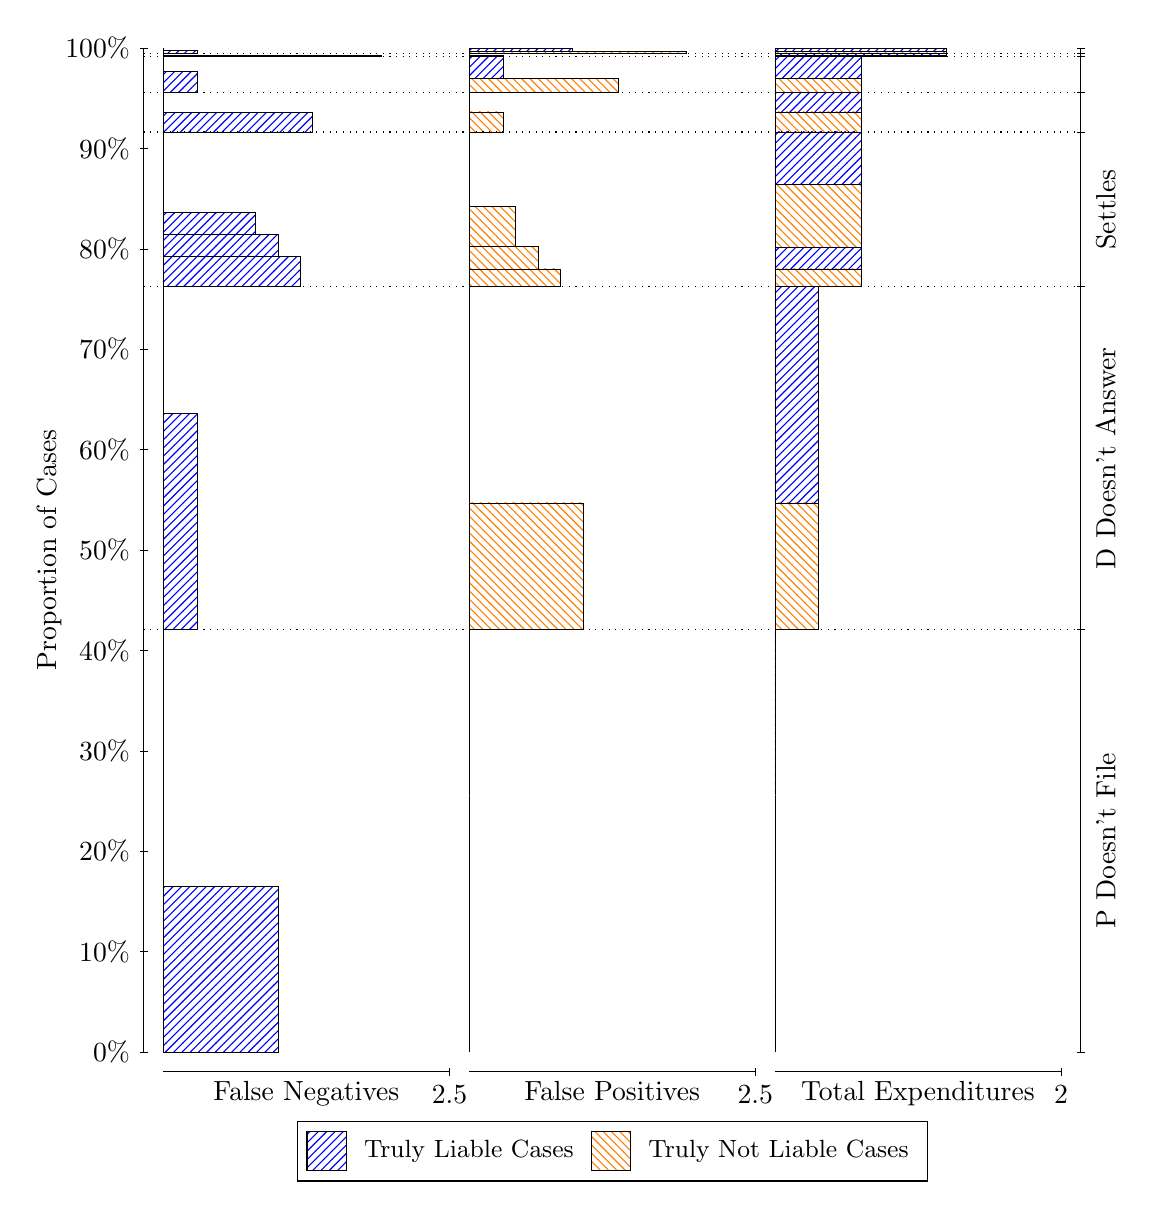
\begin{tikzpicture}
\draw[black, very thin] (1.5,1.75) -- (1.5,14.5);
\node[rotate=90, text=black, anchor=center] at (0.3, 8.125) {Proportion of Cases};
\draw[black, very thin] (1.45,1.75) -- (1.55,1.75);
\node[text=black, anchor=east] at (1.45, 1.75) {0\%};
\draw[black, very thin] (1.45,3.025) -- (1.55,3.025);
\node[text=black, anchor=east] at (1.45, 3.025) {10\%};
\draw[black, very thin] (1.45,4.3) -- (1.55,4.3);
\node[text=black, anchor=east] at (1.45, 4.3) {20\%};
\draw[black, very thin] (1.45,5.575) -- (1.55,5.575);
\node[text=black, anchor=east] at (1.45, 5.575) {30\%};
\draw[black, very thin] (1.45,6.85) -- (1.55,6.85);
\node[text=black, anchor=east] at (1.45, 6.85) {40\%};
\draw[black, very thin] (1.45,8.125) -- (1.55,8.125);
\node[text=black, anchor=east] at (1.45, 8.125) {50\%};
\draw[black, very thin] (1.45,9.4) -- (1.55,9.4);
\node[text=black, anchor=east] at (1.45, 9.4) {60\%};
\draw[black, very thin] (1.45,10.675) -- (1.55,10.675);
\node[text=black, anchor=east] at (1.45, 10.675) {70\%};
\draw[black, very thin] (1.45,11.95) -- (1.55,11.95);
\node[text=black, anchor=east] at (1.45, 11.95) {80\%};
\draw[black, very thin] (1.45,13.225) -- (1.55,13.225);
\node[text=black, anchor=east] at (1.45, 13.225) {90\%};
\draw[black, very thin] (1.45,14.5) -- (1.55,14.5);
\node[text=black, anchor=east] at (1.45, 14.5) {100\%};

\draw[black, very thin] (13.4,1.75) -- (13.4,14.5);
\draw[black, very thin] (13.35,1.75) -- (13.45,1.75);
\node[anchor=west] at (13.35, 1.75) {};
\draw[black, very thin] (13.35,7.114) -- (13.45,7.114);
\node[anchor=west] at (13.35, 7.114) {};
\draw[black, very thin] (13.35,11.469) -- (13.45,11.469);
\node[anchor=west] at (13.35, 11.469) {};
\draw[black, very thin] (13.35,13.434) -- (13.45,13.434);
\node[anchor=west] at (13.35, 13.434) {};
\draw[black, very thin] (13.35,13.937) -- (13.45,13.937);
\node[anchor=west] at (13.35, 13.937) {};
\draw[black, very thin] (13.35,14.39) -- (13.45,14.39);
\node[anchor=west] at (13.35, 14.39) {};
\draw[black, very thin] (13.35,14.429) -- (13.45,14.429);
\node[anchor=west] at (13.35, 14.429) {};
\draw[black, very thin] (13.35,14.5) -- (13.45,14.5);
\node[anchor=west] at (13.35, 14.5) {};

\draw[black, very thin, pattern color=blue, pattern=north east lines] (1.75,1.75) rectangle (3.2033,3.8558);
\draw[black, very thin, pattern color=orange, pattern=north west lines] (1.75,3.8558) rectangle (1.75,7.114);
\draw[black, very thin, pattern color=blue, pattern=north east lines] (1.75,7.114) rectangle (2.186,9.8599);
\draw[black, very thin, pattern color=orange, pattern=north west lines] (1.75,9.8599) rectangle (1.75,11.469);
\draw[black, very thin, pattern color=blue, pattern=north east lines] (1.75,11.469) rectangle (3.494,11.857);
\draw[black, very thin, pattern color=blue, pattern=north east lines] (1.75,11.857) rectangle (3.2033,12.138);
\draw[black, very thin, pattern color=blue, pattern=north east lines] (1.75,12.138) rectangle (2.9127,12.412);
\draw[black, very thin, pattern color=orange, pattern=north west lines] (1.75,12.412) rectangle (1.75,13.434);
\draw[black, very thin, pattern color=blue, pattern=north east lines] (1.75,13.434) rectangle (3.6393,13.683);
\draw[black, very thin, pattern color=orange, pattern=north west lines] (1.75,13.683) rectangle (1.75,13.937);
\draw[black, very thin, pattern color=blue, pattern=north east lines] (1.75,13.937) rectangle (2.186,14.208);
\draw[black, very thin, pattern color=orange, pattern=north west lines] (1.75,14.208) rectangle (1.75,14.39);
\draw[black, very thin, pattern color=blue, pattern=north east lines] (1.75,14.39) rectangle (4.5113,14.409);
\draw[black, very thin, pattern color=orange, pattern=north west lines] (1.75,14.409) rectangle (1.75,14.429);
\draw[black, very thin, pattern color=blue, pattern=north east lines] (1.75,14.429) rectangle (2.186,14.47);
\draw[black, very thin, pattern color=orange, pattern=north west lines] (1.75,14.47) rectangle (1.75,14.5);
\draw[black, very thin, pattern color=orange, pattern=north west lines] (5.6333,1.75) rectangle (5.6333,5.0082);
\draw[black, very thin, pattern color=blue, pattern=north east lines] (5.6333,5.0082) rectangle (5.6333,7.114);
\draw[black, very thin, pattern color=orange, pattern=north west lines] (5.6333,7.114) rectangle (7.0867,8.7227);
\draw[black, very thin, pattern color=blue, pattern=north east lines] (5.6333,8.7227) rectangle (5.6333,11.469);
\draw[black, very thin, pattern color=orange, pattern=north west lines] (5.6333,11.469) rectangle (6.796,11.694);
\draw[black, very thin, pattern color=orange, pattern=north west lines] (5.6333,11.694) rectangle (6.5053,11.982);
\draw[black, very thin, pattern color=orange, pattern=north west lines] (5.6333,11.982) rectangle (6.2147,12.49);
\draw[black, very thin, pattern color=blue, pattern=north east lines] (5.6333,12.49) rectangle (5.6333,13.434);
\draw[black, very thin, pattern color=orange, pattern=north west lines] (5.6333,13.434) rectangle (6.0693,13.688);
\draw[black, very thin, pattern color=blue, pattern=north east lines] (5.6333,13.688) rectangle (5.6333,13.937);
\draw[black, very thin, pattern color=orange, pattern=north west lines] (5.6333,13.937) rectangle (7.5227,14.119);
\draw[black, very thin, pattern color=blue, pattern=north east lines] (5.6333,14.119) rectangle (6.0693,14.39);
\draw[black, very thin, pattern color=orange, pattern=north west lines] (5.6333,14.39) rectangle (6.0693,14.41);
\draw[black, very thin, pattern color=blue, pattern=north east lines] (5.6333,14.41) rectangle (5.6333,14.429);
\draw[black, very thin, pattern color=orange, pattern=north west lines] (5.6333,14.429) rectangle (8.3947,14.459);
\draw[black, very thin, pattern color=blue, pattern=north east lines] (5.6333,14.459) rectangle (6.9413,14.5);
\draw[black, very thin, pattern color=orange, pattern=north west lines] (9.5167,1.75) rectangle (9.5167,5.0082);
\draw[black, very thin, pattern color=blue, pattern=north east lines] (9.5167,5.0082) rectangle (9.5167,7.114);
\draw[black, very thin, pattern color=orange, pattern=north west lines] (9.5167,7.114) rectangle (10.062,8.7227);
\draw[black, very thin, pattern color=blue, pattern=north east lines] (9.5167,8.7227) rectangle (10.062,11.469);
\draw[black, very thin, pattern color=orange, pattern=north west lines] (9.5167,11.469) rectangle (10.607,11.694);
\draw[black, very thin, pattern color=blue, pattern=north east lines] (9.5167,11.694) rectangle (10.607,11.968);
\draw[black, very thin, pattern color=orange, pattern=north west lines] (9.5167,11.968) rectangle (10.607,12.765);
\draw[black, very thin, pattern color=blue, pattern=north east lines] (9.5167,12.765) rectangle (10.607,13.434);
\draw[black, very thin, pattern color=orange, pattern=north west lines] (9.5167,13.434) rectangle (10.607,13.688);
\draw[black, very thin, pattern color=blue, pattern=north east lines] (9.5167,13.688) rectangle (10.607,13.937);
\draw[black, very thin, pattern color=orange, pattern=north west lines] (9.5167,13.937) rectangle (10.607,14.119);
\draw[black, very thin, pattern color=blue, pattern=north east lines] (9.5167,14.119) rectangle (10.607,14.39);
\draw[black, very thin, pattern color=orange, pattern=north west lines] (9.5167,14.39) rectangle (11.697,14.41);
\draw[black, very thin, pattern color=blue, pattern=north east lines] (9.5167,14.41) rectangle (11.697,14.429);
\draw[black, very thin, pattern color=orange, pattern=north west lines] (9.5167,14.429) rectangle (11.697,14.459);
\draw[black, very thin, pattern color=blue, pattern=north east lines] (9.5167,14.459) rectangle (11.697,14.5);
\draw[black, dotted] (1.5,7.114) -- (13.4,7.114);
\draw[black, dotted] (1.5,11.469) -- (13.4,11.469);
\draw[black, dotted] (1.5,13.434) -- (13.4,13.434);
\draw[black, dotted] (1.5,13.937) -- (13.4,13.937);
\draw[black, dotted] (1.5,14.39) -- (13.4,14.39);
\draw[black, dotted] (1.5,14.429) -- (13.4,14.429);
\draw[black, very thin] (1.75,1.5) -- (5.3833,1.5);
\node[text=black, anchor=north] at (3.5667, 1.5) {False Negatives};
\draw[black, very thin] (5.3833,1.45) -- (5.3833,1.55);
\node[text=black, anchor=north] at (5.3833, 1.45) {2.5};

\draw[black, very thin] (5.6333,1.5) -- (9.2667,1.5);
\node[text=black, anchor=north] at (7.45, 1.5) {False Positives};
\draw[black, very thin] (9.2667,1.45) -- (9.2667,1.55);
\node[text=black, anchor=north] at (9.2667, 1.45) {2.5};

\draw[black, very thin] (9.5167,1.5) -- (13.15,1.5);
\node[text=black, anchor=north] at (11.333, 1.5) {Total Expenditures};
\draw[black, very thin] (13.15,1.45) -- (13.15,1.55);
\node[text=black, anchor=north] at (13.15, 1.45) {2};

\node[text=black, centered, rotate=90] at (13.72, 4.432) {P Doesn't File};
\node[text=black, centered, rotate=90] at (13.72, 9.2913) {D Doesn't Answer};
\node[text=black, centered, rotate=90] at (13.72, 12.451) {Settles};





\draw (7.449999999999999,1.5) node[draw=none] (baseCoordinate) {};
\begin{scope}[align=center]
        \matrix[scale=0.5, draw=black, below=0.5cm of baseCoordinate, nodes={draw}, column sep=0.1cm]{
            \node[rectangle, draw, minimum width=0.5cm, minimum height=0.5cm, pattern color=blue, pattern=north east lines] {}; &
            \node[draw=none, font=\small, text=black] (B) {Truly Liable Cases}; &
            \node[rectangle, draw, minimum width=0.5cm, minimum height=0.5cm, pattern color=orange, pattern=north west lines] {}; &
            \node[draw=none, font=\small, text=black] (B) {Truly Not Liable Cases}; \\
            };
\end{scope}

\end{tikzpicture}
\end{document}